\section{Theorie}
\label{sec:Theorie}
Aufgrund der hohen Präzision werden üblicherwiese Brückenschaltungen eingesetzt. Um die Präzision zu gewährleisten wird die sogenannte Nullmethode eingesetzt.
Mit Hilfe dieser Methode werden die Schaltungen abgeglichen, damit die zu messenden Größen mit einer hohen Genauigkeit bestimmt werden können. Außerdem lässt sich jede
physikalische Größem, welche sich als elektrischer Widerstand darstellen lässt, sehr präzise messen.
\subsection{Allgmeine Brückenschaltung}
Um die Ableichbedigung zu berechnen, betrachtet man zunächst die Spannung zwischen zwei Punkten auf zwei verschieden Leitern. Die dort anliegende Potentialdifferenz U
zwischen den Punkten A und B, welche auch als Brückenspannung bezeichnet wird hängt von den Widerstandsverhältnissen ab,
weswegen man dieses Verhätnis zum Abgleichen ausnutzt.
Die allgemeine Gestalt einer Brückenschaltung wird in  Abbildung \ref{fig:allgBrücke}
\begin{figure}
    \centering
    \caption{Allgemeine Brückenschaltung} 
    \label{fig:allgBrücke}
    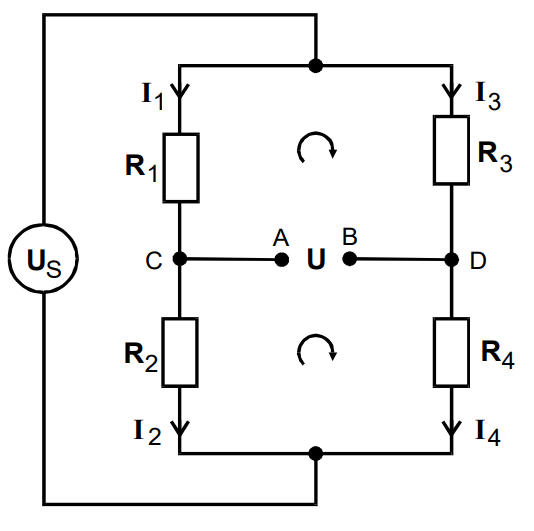
\includegraphics[width = 0.5\textwidth]{bridges/genbridge.png}
\end{figure}
dargestellt. Allgemein kann man Schaltkreise mit Hilfe der Kirchhoffschen Gesetzen beschreiben.
\subsection{Kirchoffschen Gesetze}
\subsubsection{Knotenregel}
Die erste Kirchhoffsche Regel ist die Knotenregel, welche besagt, dass die Summe aus den zufließenden und abfließenden Strömen Null ist.
Mathematisch ausgedrückt sieht die Knotenregel wie foglt aus:
\begin{equation}
    \sum_{k=1}^N I_k = 0 \label{eqn:knotrule}
\end{equation} 
\begin{figure}
    \centering
    \caption{Illustration zur Knotenregel}
    \label{fig:knotrule}
    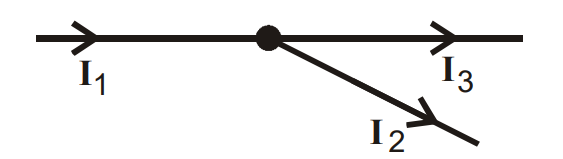
\includegraphics[width = 0.5\textwidth]{bridges/knotrule.png}
\end{figure}
Damit die Konfiguration in Abbildung \ref{fig:knotrule} gültig ist, müssen entweder die abfließenden Ströme $I_2$ und $I_3$ oder 
der zufließende Strom $I_1$ ein negatives Vorzeichen haben, so dass die Gleichung \eqref{eqn:knotrule} ihre Gültigkeit 
behält. Zwecks Konventionen besitzen die abfließenden Ströme negative Vorzeichen.
\subsubsection{Maschenregel}
Die zweite und damit letzte Kirchhoffsche Regel sagt aus, dass die Summe der Spannungen in einer sogenannten Masche ebenfalls Null ergeben muss, so dass sich die Formel
\begin{equation}
    \sum_{k=1}^N U_k = 0 \label{eqn:stitchrule}
\end{equation}
ergibt.
\begin{figure}
    \centering
    \caption{Illustration zur Maschenregel}
    \label{fig:stitchrule}
    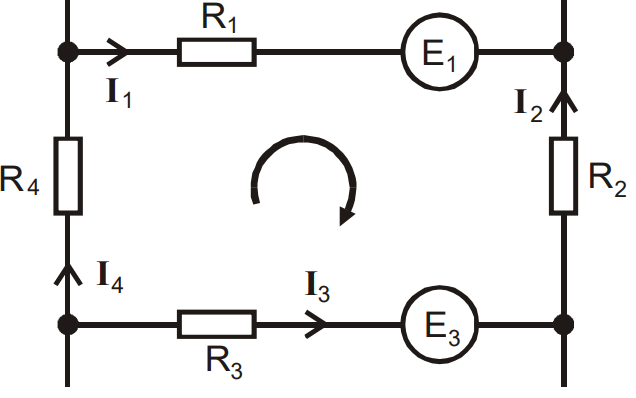
\includegraphics[width=0.5\textwidth]{bridges/stitchrule.png}
\end{figure}
Hierbei müssen manche manche Spannung über die jeweiligen Komponenten ein negatives Vorzeichen besitzen, damit die Gleichung \eqref{eqn:stitchrule} aufgeht.
Die Spannungen, wessen Pfeile des Stroms gegen den Uhrzeigersinn laufen, erhalten ein negative Vorzeichen.
\subsection{Abgleichbedingung}
Damit die Größen der gesuchten Bauteile errechnen werden können, muss die Brücke abgeglichen sein. Dies bedeutet, dass die Spannung U zwischen den Punkten A und B (s. 
Abbildung \ref{fig:allgBrücke}) gleich Null ist. Um zu messen, wie groß die Spannung U ist, benötigt wird ein Nullindikator benötigt.
Nach Anwendung der beiden Kirchhoffschen Gesetzen erhält ergibt sich für $U_\text{S}$ der Ausdruck  
\begin{equation}
    U = \frac{R_2 R_3 - R_1 R_4}{\left( R_3 + R_4 \right) \left( R_1 + R_2\right)} U_\text{S} \; \text{.} \label{eqn:matchingcondition}
\end{equation}
Damit die Spannung U verschwindet, muss der Zähler aus Gleichung \eqref{eqn:matchingcondition} Null ergeben, so dass sich die Abgleichbedigung mathematisch zu
\begin{equation}
    R_1 R_4 = R_2 R_3 \label{fig:matchingcondition}
\end{equation}
zusammenfassen lässt. 
\subsection{Wheatstonesche Brücke}
Um einen unbekannten Ohmschen Widerstand $R_\text{x}$ auszumessen, kann die Wheatstonesche Brücke benutzt werden. 
\begin{figure}
    \centering
    \caption{Schaltskizze der Wheatstonschen Brücke}
    \label{fig:Wheatstone}
    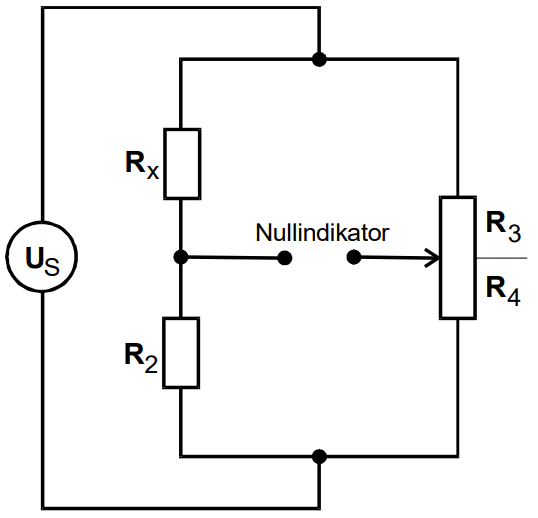
\includegraphics[width = 0.5\textwidth]{bridges/wheat.png}
\end{figure}
Die Formel für den unbekannte Widerstand $R_x$ lässt sich mit Hilfe der Abgleichbedigung \eqref{eqn:matchingcondition} durch umstellen errechnen. Somit folgt 
\begin{equation}
    R_\text{x} = R_2 \frac{R_3}{R_4} \; \text{.} \label{eqn:wheat}
\end{equation}
\subsection{Kapazitätsmessbrücke} \label{subsec:capmesbridge}
\begin{figure}
    \centering  
    \caption{Schaltskizze einer Kapazitätsmessbrücke}
    \label{fig:capmesbridge}
    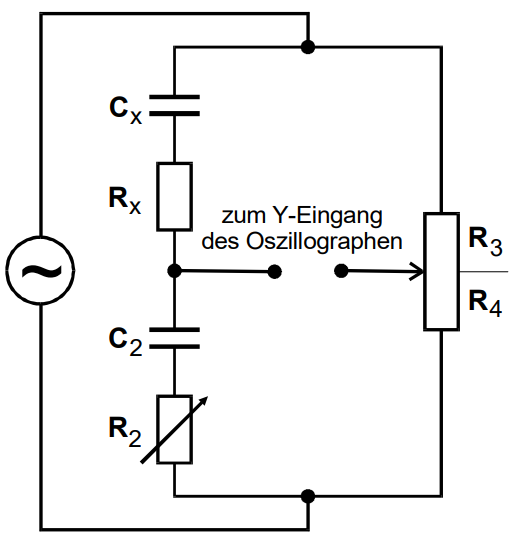
\includegraphics[width = 0.5\textwidth]{bridges/capmesbridge.png}
\end{figure}
Die Eigenschaft, dass bei einer Kapazität Arbeit gegen den Strom verrichtet wird und somit ein Teil der Energie in Wärmeenergie verloren geht, muss, um ein genaues
Ergebnis zu erzielen, diese Verlustenergie mit berücksichtigt werden. Um diese meist unerwünschte Eigenschaft zu realisieren, wird ein Ersatzwiderstand 
hinter die Kapazität geschaltet. Somit wird der Energieverlust bei der Berechnung berücksichtigt. Mit der Ersatzschaltung ergibt sich die Schaltskizze 
für die Kapazitätsmessbrücke \ref{fig:capmesbridge}. Die Formeln für die Berechnung der unbekannten Größen $R_x$ und $C_x$ sind einerseits in Gleichung
\eqref{eqn:wheat} und ergeben sich aus 
\begin{equation}
    C_x = C_2 \frac{R_4}{R_3}
\end{equation}
\subsection{Induktivitätsmessbrücke} \label{subsec:inductance}
Ähnlich wie bei der Kapazitätsmessbrücke \ref{subsec:capmesbridge} geht aufgrund der Spule Energie verloren.
Dies geschieht, da diese einen Teil ihrer magnetischen Feldenergie in Form von Wärmeenergie an die Umwelt abgibt. Somit wird erneut ein Verlustwiderstand 
hinter das jeweilige Bauteil(in diesem Fall eine Induktivität) geschaltet, sodass der Versuchsaufbau realistisch ist.
\begin{figure}
    \centering
    \caption{Schaltskizze einer Induktivitätsmessbrücke}
    \label{fig:inductance}
    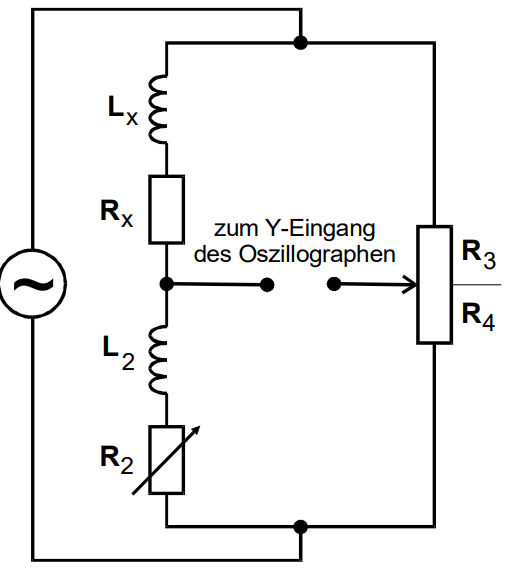
\includegraphics[width=0.5\textwidth]{bridges/inductance.png}
\end{figure}
Die zur Berechnung der unbekannten Größen $R_x$ und $L_x$ nötigen Formeln sind erneut einerseits durch Gleichung \eqref{eqn:wheat}
und durch
\begin{equation}
    L_x = L_2 \frac{R_3}{R_4}
\end{equation}
gegeben.
\subsection{Maxwell-Brücke}
Die Maxwell-Brücke dient ebenfalls zur Induktivitätsmessung. Oftmals wird diese Brückenschaltung genutzt, da diese gegenüber der oben erwähnten Brücken
schaltung \ref{subsec:inductance}den Vorteil besitzt, dass die Induktivität $L_2$ einen nicht so niedrigen Verlust haben muss. Dies ist ein großer Vorteil, da eine 
effiziente Spule schwer zu realisieren ist.
\begin{figure}
    \centering
    \caption{Schaltskizze der Maxwell-Brücke}
    \label{fig:maxwell}
    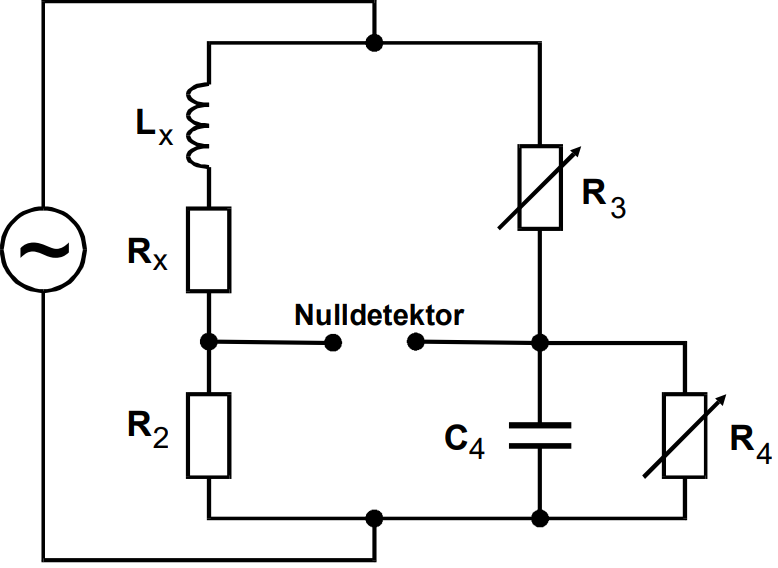
\includegraphics[width=0.5\textwidth]{bridges/maxwell.png}
\end{figure}
Hierbei werden die Regelwiderstände $R_3$ und $R_4$ als Abgleichelemente genutzt. Bei diesem Versuchsaufbau ist die Kapazität $C_4$ eine möglichst verlustfreie 
Kapazität. Zur Berechnung der gesuchten Größen $R_x$ und $L_x$ dient erneut die Gleichung \eqref{eqn:wheat} und die Formel
\begin{equation}
    L_x = R_2 R_3 C_4
\end{equation}
\subsection{Wien-Robinson-Brücke}
Die Wien-Robinson-Brücke ist im Gegensatz zu den vorigen Brücken eine frequenzabhängige Brücke, bei welcher die Durchführung nur bei eine Frequenz möglich ist.
Außerdem besitzt diese Brücke keine Abgleichelemente.
\begin{figure}
    \centering
    \caption{Schaltskizze der Wien-Robinson-Brücke}
    \label{fig:WR}
    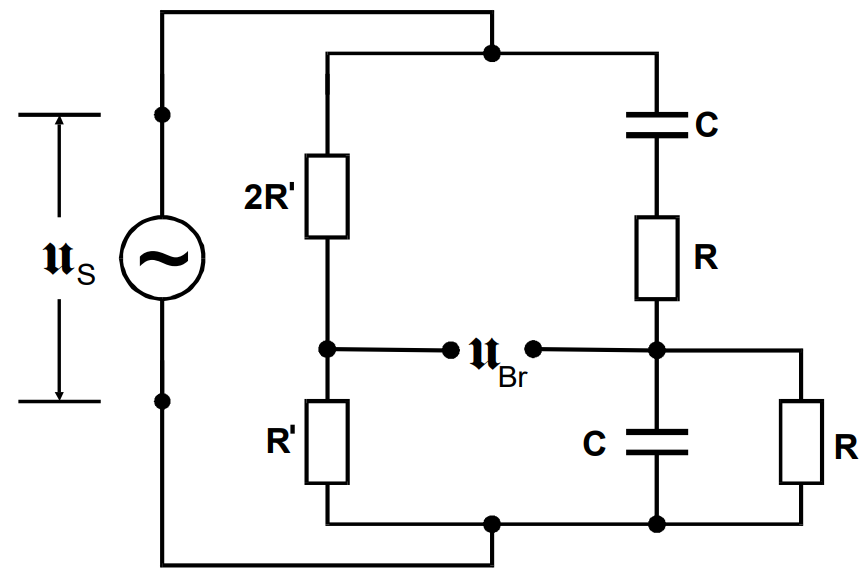
\includegraphics[width=0.5\textwidth]{bridges/WR.png}
\end{figure}
Für den Betrag der Brücken- und Speisepannung gilt
\begin{equation}
    \abs*{\frac{U_B}{U_S}}^2 = \frac{1}{9} \frac{\left(\omega^2 R^2 C^2 -1 \right)^2}{\left( \left( 1 - \omega^2 R^2 C^2 \right)^2 
    + 9 w^2 R^2 C^2 \right)}
\end{equation}
Die Brückenspannung verschwindet bei der Frequenz 
\begin{equation}
    \omega_0 = 1/RC
\end{equation}
, wodurch die Brücke bei der Frequenz $\omega_0$ abgeglichen ist.
Mit $\Omega \coloneq \frac{\omega}{\omega_0}$ erhält man 
\begin{equation}
    f(\Omega) = \abs*{\frac{U_B}{U_S}}^2 = \frac{1}{9} \frac{\left(\Omega^2 -1 \right)^2}{ \left( 1 - \Omega^2 R^2 \right)^2 
    + 9 \Omega^2}
\end{equation}
Der Klirrfaktor $k$ wird mittels
\begin{equation}
    k = \sqrt{\frac{U_2^2 + U_3^2 + \dotsb }{U_1^2}}
\end{equation}
errechnet. Als Vereinfachung wir nur die Spannung $U_2$ der ersten Oberwelle mit einbezogen. Somit ergibt sich
\begin{equation}
    k = \frac{U_2}{U_1} \; \text{.}
\end{equation} 
Die Spannung $U_2$ erhält man mit Hilfe von 
\begin{equation}
    U_2 = \frac{U_B}{f(\Omega = 2)} \; \text{.}
\end{equation}